\documentclass[12pt,a4paper]{article}

\makeatletter
    \usepackage[utf8]{inputenc}
\usepackage[T1]{fontenc}
\usepackage{ucs}

\usepackage[french]{babel,varioref}

\usepackage[top=2cm, bottom=2cm, left=1.5cm, right=1.5cm]{geometry}
\usepackage{enumitem}

\usepackage{multicol}

\usepackage{makecell}

\usepackage{color}
\usepackage{hyperref}
\hypersetup{
    colorlinks,
    citecolor=black,
    filecolor=black,
    linkcolor=black,
    urlcolor=black
}

\usepackage{amsthm}

\usepackage{tcolorbox}
\tcbuselibrary{listingsutf8}

\usepackage{ifplatform}

\usepackage{ifthen}

\usepackage{cbdevtool}


% MISC

\newtcblisting{latexex}{%
	sharp corners,%
	left=1mm, right=1mm,%
	bottom=1mm, top=1mm,%
	colupper=red!75!blue,%
	listing side text
}

\newtcblisting{latexex-flat}{%
	sharp corners,%
	left=1mm, right=1mm,%
	bottom=1mm, top=1mm,%
	colupper=red!75!blue,%
}

\newtcblisting{latexex-alone}{%
	sharp corners,%
	left=1mm, right=1mm,%
	bottom=1mm, top=1mm,%
	colupper=red!75!blue,%
	listing only
}


\newcommand\env[1]{\texttt{#1}}
\newcommand\macro[1]{\env{\textbackslash{}#1}}



\setlength{\parindent}{0cm}
\setlist{noitemsep}

\theoremstyle{definition}
\newtheorem*{remark}{Remarque}

\usepackage[raggedright]{titlesec}

\titleformat{\paragraph}[hang]{\normalfont\normalsize\bfseries}{\theparagraph}{1em}{}
\titlespacing*{\paragraph}{0pt}{3.25ex plus 1ex minus .2ex}{0.5em}


\newcommand\separation{
	\medskip
	\hfill\rule{0.5\textwidth}{0.75pt}\hfill
	\medskip
}


\newcommand\extraspace{
	\vspace{0.25em}
}


\newcommand\whyprefix[2]{%
	\textbf{\prefix{#1}}-#2%
}

\newcommand\mwhyprefix[2]{%
	\texttt{#1 = #1-#2}%
}

\newcommand\prefix[1]{%
	\texttt{#1}%
}


\newcommand\inenglish{\@ifstar{\@inenglish@star}{\@inenglish@no@star}}

\newcommand\@inenglish@star[1]{%
	\emph{\og #1 \fg}%
}

\newcommand\@inenglish@no@star[1]{%
	\@inenglish@star{#1} en anglais%
}


\newcommand\ascii{\texttt{ASCII}}


% Example
\newcounter{paraexample}[subsubsection]

\newcommand\@newexample@abstract[2]{%
	\paragraph{%
		#1%
		\if\relax\detokenize{#2}\relax\else {} -- #2\fi%
	}%
}



\newcommand\newparaexample{\@ifstar{\@newparaexample@star}{\@newparaexample@no@star}}

\newcommand\@newparaexample@no@star[1]{%
	\refstepcounter{paraexample}%
	\@newexample@abstract{Exemple \theparaexample}{#1}%
}

\newcommand\@newparaexample@star[1]{%
	\@newexample@abstract{Exemple}{#1}%
}


% Change log
\newcommand\topic{\@ifstar{\@topic@star}{\@topic@no@star}}

\newcommand\@topic@no@star[1]{%
	\textbf{\textsc{#1}.}%
}

\newcommand\@topic@star[1]{%
	\textbf{\textsc{#1} :}%
}






    % == PACKAGES USED == %

\RequirePackage{amsmath}
\RequirePackage{relsize}
\RequirePackage{xparse}


% == DEFINITIONS == %

% Settable texts
\@ifpackagewith{babel}{french}{
    \newcommand\lymathsep{;}
    \newcommand\lymathsubsep{,}

    \newcommand\textopchoice{choix}
    \newcommand\textopcond{cond}
    \newcommand\textopdef{déf}
    \newcommand\textophyp{hyp}
    \newcommand\textopid{id}
    \newcommand\textoptest{?}
}{
    \newcommand\lymathsep{,}
    \newcommand\lymathsubsep{;}

    \newcommand\textopchoice{choice}
    \newcommand\textopcond{cond}
    \newcommand\textopdef{def}
    \newcommand\textophyp{hyp}
    \newcommand\textopid{id}
    \newcommand\textoptest{?}
}


\newcommand\textexplainleft{\{}
\newcommand\textexplainright{\}}
\newcommand\textexplainspacein{2em}


% Tools - Apply same macro to all arguments

% #1        : main macro
% #2        : macro to apply to arguments
% #3 and #4 : the two arguments
\newcommand\@apply@macro@two@args[4]{%
    #1{#2{#3}}{#2{#4}}%
}


% Tools - Deco over a math symbol

\newcommand\@over@math@symbol[2]{%
	\mathrel{\overset{\mathrm{\text{\raisebox{.5ex}{#1}}}}{#2}}%
}


% Tools - Intervals

\newcommand\@extra@phantom{%
    \vphantom{\relsize{1.25}{\text{$\displaystyle F_1^2$}}}%
}

\newcommand\@interval@tool@star[5]{%
    \ensuremath{ \left#1 \@extra@phantom \right. \!\! #2 #3 #4 \left. \@extra@phantom \!\! \right#5}%
}

\newcommand\@interval@tool@no@star[5]{\ensuremath{ \left#1 #2 #3 #4 \right#5}}


% Tools - Multi-arguments
%
% Source : the following lines come directly for the following post
%
%    * https://tex.stackexchange.com/a/475291/6880

\ExplSyntaxOn
% General purpose macro for defining other macros
    \NewDocumentCommand{\makemultiargument}{mmmmmo}{
        \lymath_multiarg:nnnnnn{#1}{#2}{#3}{#4}{#5}{#6}
    }
 
% Allocate a private variable
    \seq_new:N \l__lymath_generic_seq

% The internal version of the general purpose macro
    \cs_new_protected:Nn \lymath_multiarg:nnnnnn{
        % #1 = separator
        % #2 = multiargument
        % #3 = code before
          % #4 = code between
          % #5 = code after
          % #6 = ornament to items

        % A group allows nesting
        \group_begin:
         % Split the multiargument into parts
        \seq_set_split:Nnn \l__lymath_generic_seq { #1 } { #2 }
        % Apply the ornament to the items
          \tl_if_novalue:nF { #6 }{
            \seq_set_eq:NN \l__lymath_temp_seq \l__lymath_generic_seq
            \seq_set_map:NNn \l__lymath_generic_seq \l__lymath_generic_seq { #6 }
           }
        % Execute the <code before>
          #3
        % Deliver the items, with the chosen material between them
          \seq_use:Nn \l__lymath_generic_seq { #4 }
          % Execute the <code after>
         #5
          % End the group started at the beginning
          \group_end:
    }    
\ExplSyntaxOff


    \usepackage{06-demo-explained}
\makeatother


\newcommand\anglein[1]{#1}

\begin{document}

%\section{Logique et fondements}

%\subsection{Détailler un \og vrai \fg{} raisonnement}

\subsubsection{Un tableau pour le collège et le lycée} \label{explain-hard-proof-for-youngs}


\newparaexample{Avec les réglages par défaut}

L'environnement étoilé \env{demoexplain*} est différent de l'environnement \env{demoexplain} puisqu'il sert à indiquer trois choses et non juste deux comme le montre l'exemple suivant
\footnote{
	C'est pour cela qu'est proposé une version étoilée de l'environnement et non l'utilisation d'une option de l'environnement non étoilé. 
}.
Par contre, la syntaxe est très similaire.
Notez au passage la possibilité d'utiliser \macro{newline} pour forcer un retour à la ligne dans une cellule.

\begin{latexex-flat}
\begin{demoexplain*}
    \demostep
        $ABC$ est un triangle
        \newline équilatéral 
      & Dans un triangle équilatéral, les trois angles mesurent $60$\textdegree. 
      & $\anglein{ABC} = 60$\textdegree     
    \demostep
        Voir la conséquence \explref*{1} .
      & Simple calcul avec conversion en radians.
      & $\dfrac{1}{3} \anglein{ABC} = \dfrac{\pi}{9}$
\end{demoexplain*}
\end{latexex-flat}


% ---------------------- %


\newparaexample{Avec toutes les options}

Le système de référence marche ici aussi.
Par contre \env{demoexplain*} ne propose que \verb+start+ comme clé optionnelle avec le même fonctionnement que pour \env{demoexplain}.

\begin{latexex-flat}
\begin{demoexplain*}[start = last]
    \demostep[demo-first-geo-fact]
        $ABC$ est un triangle \newline équilatéral 
      & Dans un triangle équilatéral, les trois angles mesurent $60$\textdegree. 
      & $\anglein{ABC} = 60$\textdegree     
    \demostep
        Voir la conséquence \explref{demo-first-geo-fact} .
      & Simple calcul avec conversion en radians.
      & $\dfrac{1}{3} \anglein{ABC} = \dfrac{\pi}{9}$
\end{demoexplain*}
\end{latexex-flat}


% ---------------------- %


\subsubsection{Un tableau sur plusieurs pages}

Un tableau devant utiliser plusieurs pages sera scindé comme ci-dessous sans perte d'information
\footnote{
	Tout le travail est fait par l'environnement \env{longtable} du package éponyme.
}.

\begin{center}
	\frame{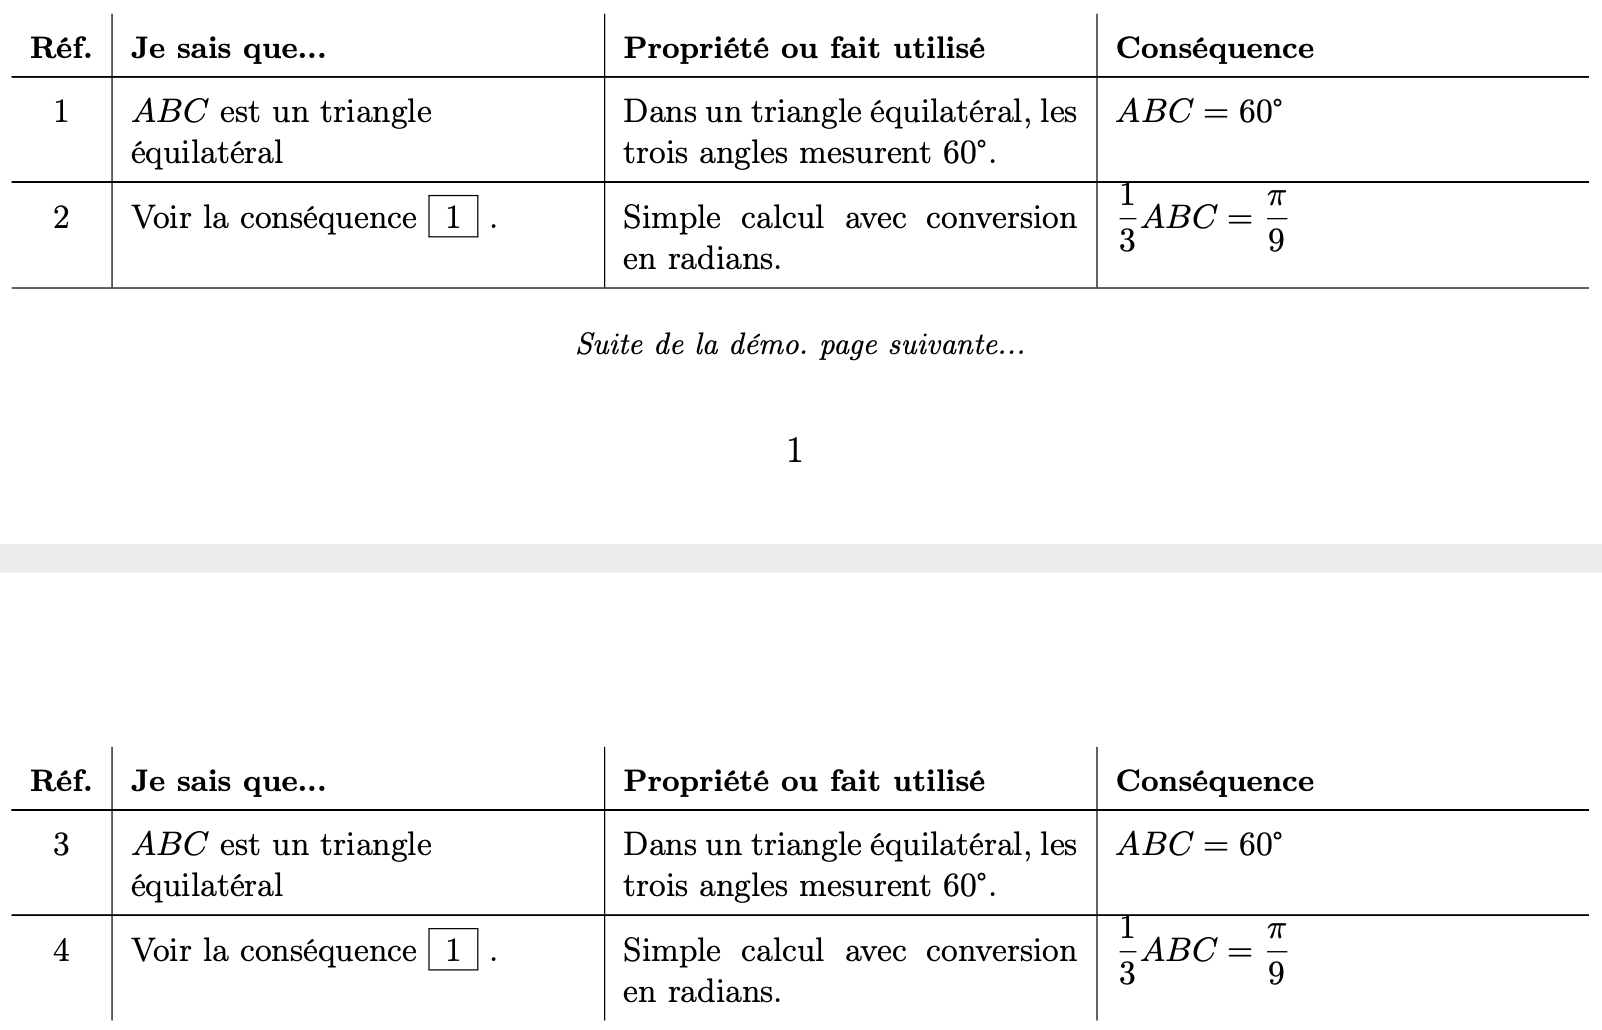
\includegraphics[scale = .5]{demo-explained-middleschool-broken[fr].png}}
\end{center}

\end{document}
